% Modelo logico do banco de dados (Figura do item 4.4.2). Gera fig_modelo_logico.png.
\documentclass[border=8pt]{standalone}
\usepackage[utf8]{inputenc}
\usepackage[T1]{fontenc}
\usepackage{tikz}
\usetikzlibrary{shapes.multipart,positioning,calc}
\definecolor{azul}{RGB}{31,98,170}
\definecolor{marrom}{RGB}{130,82,14}
\tikzset{
  tabela/.style={rectangle split, rectangle split parts=2, draw=azul, line width=0.6pt,
    rectangle split part align={center,left}, text width=6.2cm, inner sep=4pt, font=\small},
  card/.style={font=\footnotesize, text=black!65},
  rel/.style={draw=black!60, line width=0.6pt},
}
% \tabela{id}{posicao}{titulo}{cor do cabecalho}{linhas}
\newcommand{\tabela}[5]{%
  \node[tabela, rectangle split part fill={#4,white}] (#1) at #2
    {\textcolor{white}{\textbf{#3}}\nodepart{two}%
     \begin{tabular}{@{}l@{\ \ }l@{}}#5\end{tabular}};}
\newcommand{\pk}{\textbf{PK}}
\newcommand{\fk}{\textbf{FK}}
\begin{document}
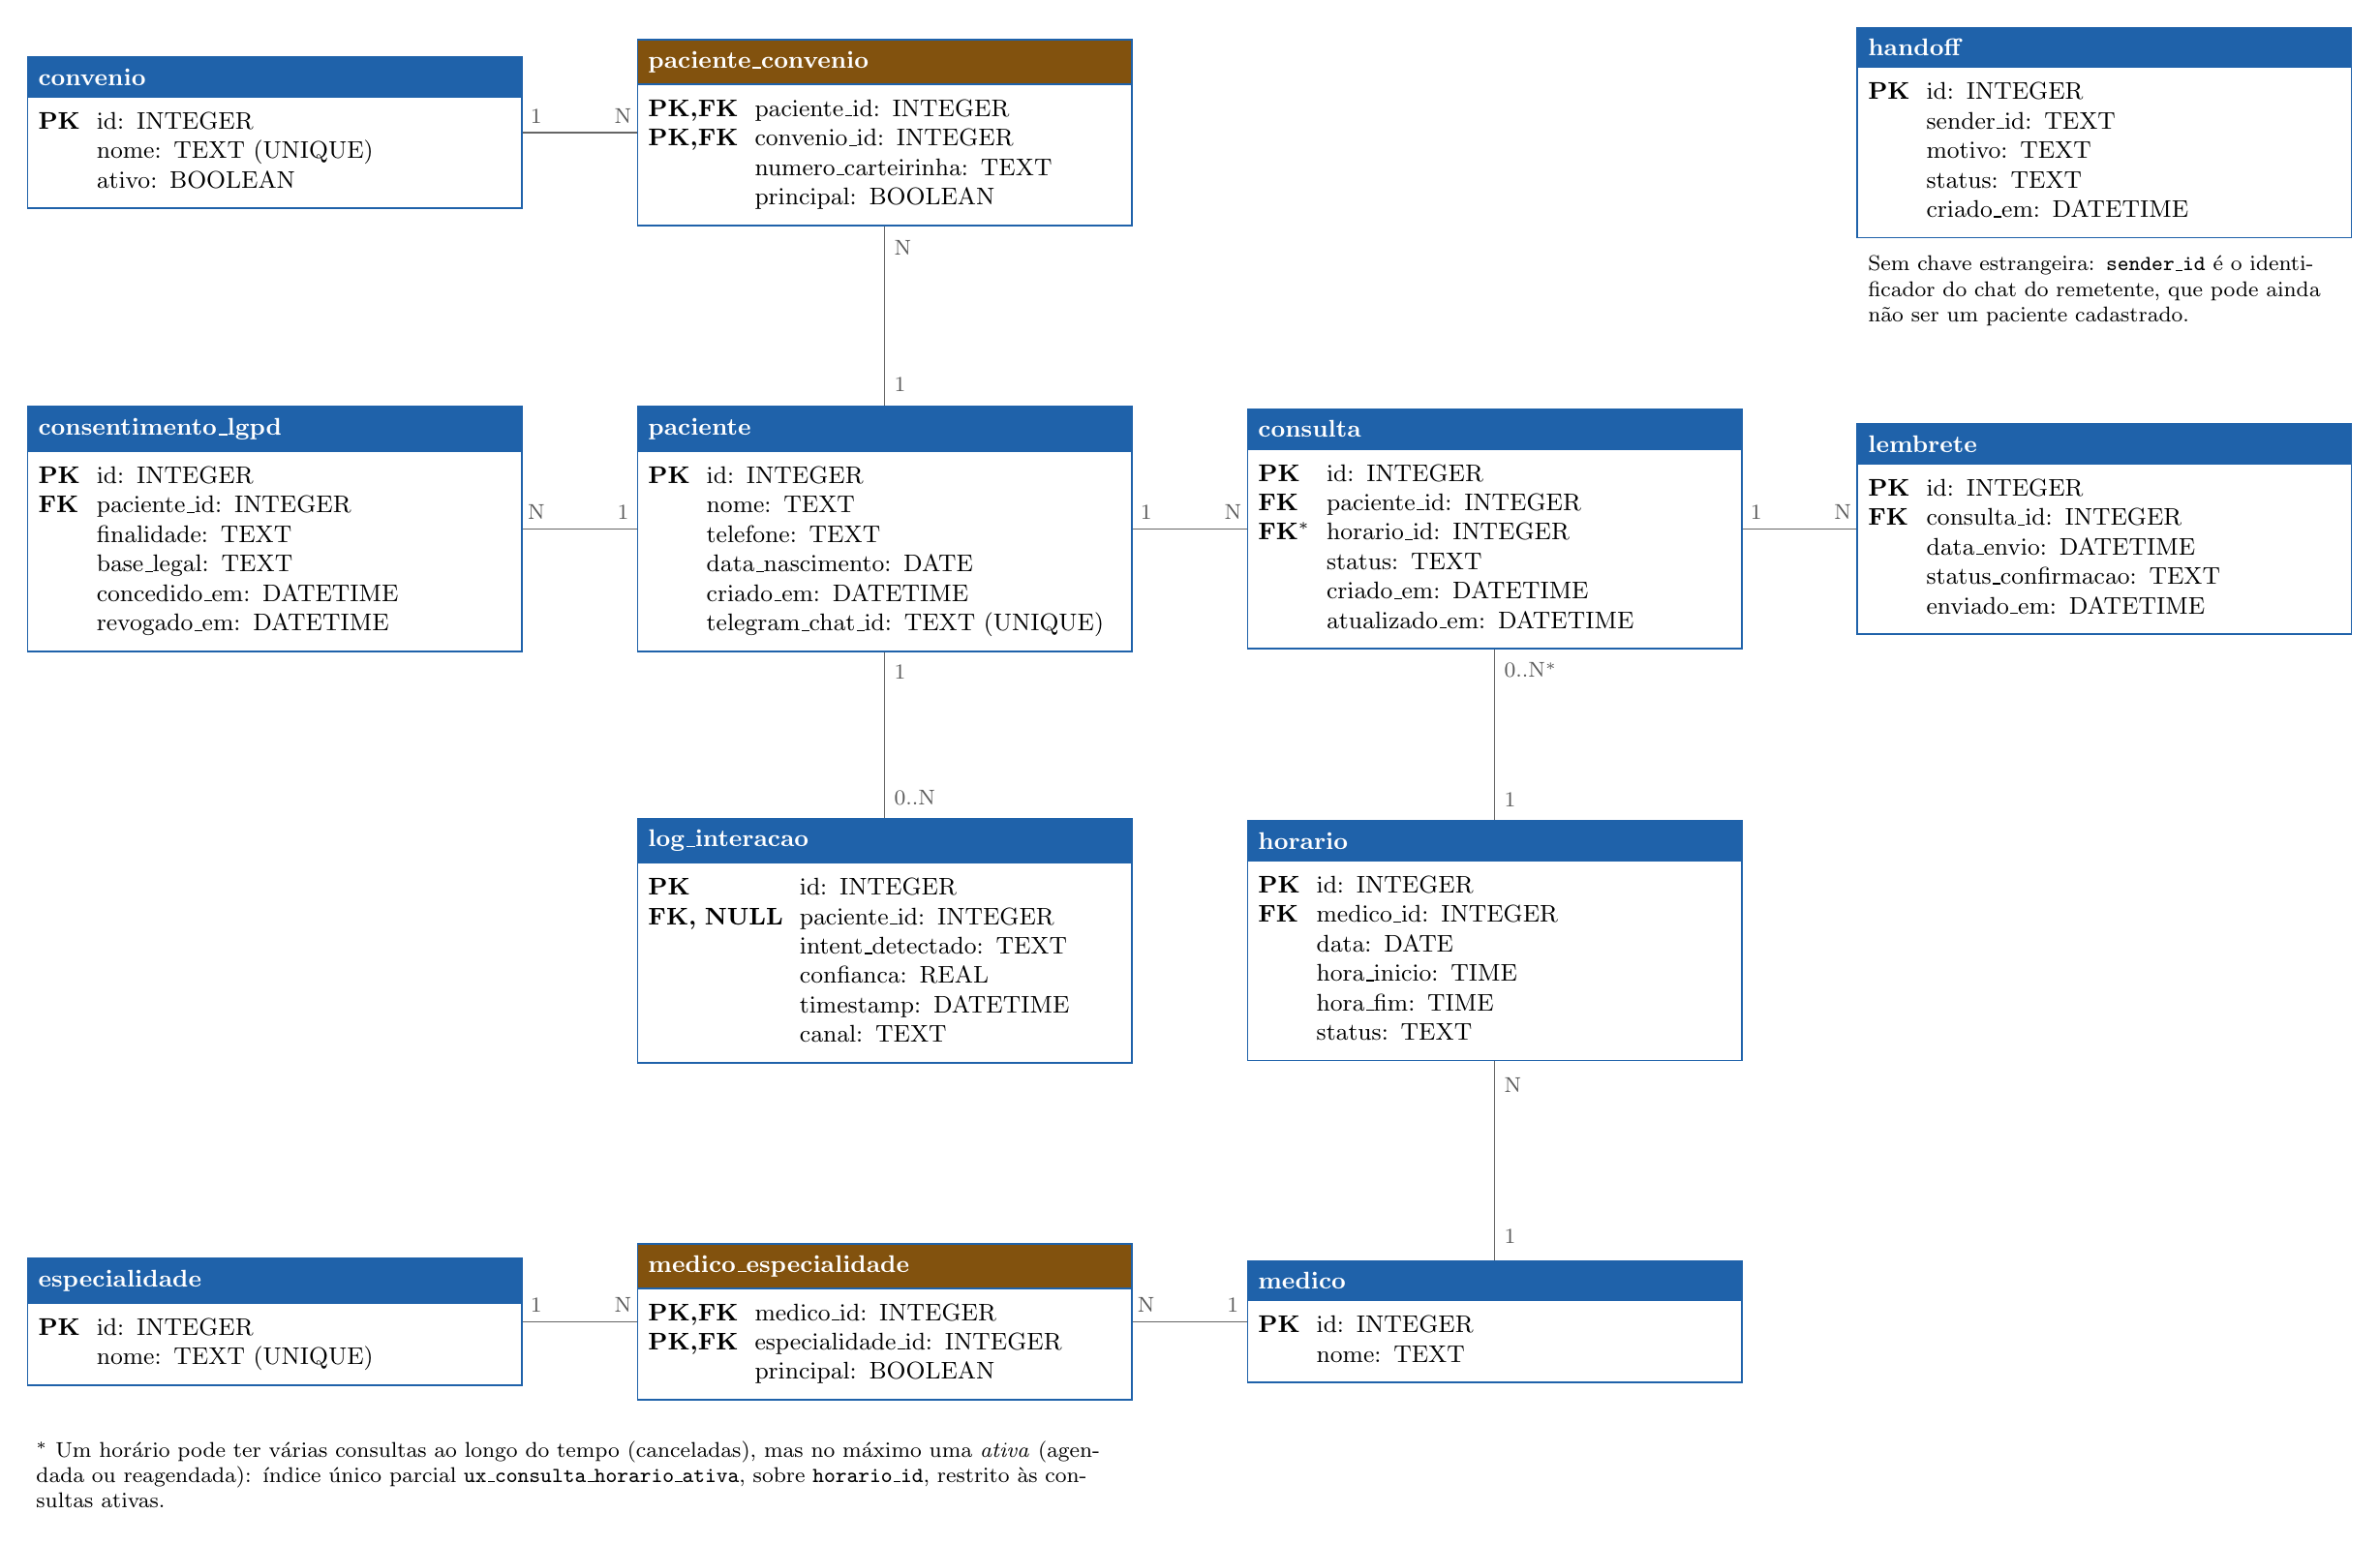
\begin{tikzpicture}
% linha 1
\tabela{convenio}{(0,0)}{convenio}{azul}{%
  \pk & id: INTEGER\\ & nome: TEXT (UNIQUE)\\ & ativo: BOOLEAN}
\tabela{pc}{(8,0)}{paciente\_convenio}{marrom}{%
  \textbf{PK,FK} & paciente\_id: INTEGER\\ \textbf{PK,FK} & convenio\_id: INTEGER\\
  & numero\_carteirinha: TEXT\\ & principal: BOOLEAN}
\tabela{handoff}{(24,0)}{handoff}{azul}{%
  \pk & id: INTEGER\\ & sender\_id: TEXT\\ & motivo: TEXT\\ & status: TEXT\\ & criado\_em: DATETIME}
% linha 2
\tabela{consent}{(0,-5.2)}{consentimento\_lgpd}{azul}{%
  \pk & id: INTEGER\\ \fk & paciente\_id: INTEGER\\ & finalidade: TEXT\\ & base\_legal: TEXT\\
  & concedido\_em: DATETIME\\ & revogado\_em: DATETIME}
\tabela{paciente}{(8,-5.2)}{paciente}{azul}{%
  \pk & id: INTEGER\\ & nome: TEXT\\ & telefone: TEXT\\ & data\_nascimento: DATE\\
  & criado\_em: DATETIME\\ & telegram\_chat\_id: TEXT (UNIQUE)}
\tabela{consulta}{(16,-5.2)}{consulta}{azul}{%
  \pk & id: INTEGER\\ \fk & paciente\_id: INTEGER\\ \textbf{FK}$^{*}$ & horario\_id: INTEGER\\
  & status: TEXT\\ & criado\_em: DATETIME\\ & atualizado\_em: DATETIME}
\tabela{lembrete}{(24,-5.2)}{lembrete}{azul}{%
  \pk & id: INTEGER\\ \fk & consulta\_id: INTEGER\\ & data\_envio: DATETIME\\
  & status\_confirmacao: TEXT\\ & enviado\_em: DATETIME}
% linha 3
\tabela{log}{(8,-10.6)}{log\_interacao}{azul}{%
  \pk & id: INTEGER\\ \textbf{FK, NULL} & paciente\_id: INTEGER\\ & intent\_detectado: TEXT\\
  & confianca: REAL\\ & timestamp: DATETIME\\ & canal: TEXT}
\tabela{horario}{(16,-10.6)}{horario}{azul}{%
  \pk & id: INTEGER\\ \fk & medico\_id: INTEGER\\ & data: DATE\\ & hora\_inicio: TIME\\
  & hora\_fim: TIME\\ & status: TEXT}
% linha 4
\tabela{especialidade}{(0,-15.6)}{especialidade}{azul}{%
  \pk & id: INTEGER\\ & nome: TEXT (UNIQUE)}
\tabela{me}{(8,-15.6)}{medico\_especialidade}{marrom}{%
  \textbf{PK,FK} & medico\_id: INTEGER\\ \textbf{PK,FK} & especialidade\_id: INTEGER\\ & principal: BOOLEAN}
\tabela{medico}{(16,-15.6)}{medico}{azul}{%
  \pk & id: INTEGER\\ & nome: TEXT}

% relacionamentos (cardinalidade junto de cada tabela)
\draw[rel] (convenio.east) -- node[card,pos=0.12,above]{1} node[card,pos=0.88,above]{N} (convenio.east -| pc.west);
\draw[rel] (pc.south) -- node[card,pos=0.12,right]{N} node[card,pos=0.88,right]{1} (paciente.north);
\draw[rel] (consent.east) -- node[card,pos=0.12,above]{N} node[card,pos=0.88,above]{1} (consent.east -| paciente.west);
\draw[rel] (paciente.east) -- node[card,pos=0.12,above]{1} node[card,pos=0.88,above]{N} (paciente.east -| consulta.west);
\draw[rel] (consulta.east) -- node[card,pos=0.12,above]{1} node[card,pos=0.88,above]{N} (consulta.east -| lembrete.west);
\draw[rel] (paciente.south) -- node[card,pos=0.12,right]{1} node[card,pos=0.88,right]{0..N} (log.north);
\draw[rel] (consulta.south) -- node[card,pos=0.12,right]{0..N$^{*}$} node[card,pos=0.88,right]{1} (horario.north);
\draw[rel] (horario.south) -- node[card,pos=0.12,right]{N} node[card,pos=0.88,right]{1} (medico.north);
\draw[rel] (especialidade.east) -- node[card,pos=0.12,above]{1} node[card,pos=0.88,above]{N} (especialidade.east -| me.west);
\draw[rel] (me.east) -- node[card,pos=0.12,above]{N} node[card,pos=0.88,above]{1} (me.east -| medico.west);

% notas
\node[font=\footnotesize, text width=6.2cm, align=left, below=3pt of handoff] {Sem chave estrangeira: \texttt{sender\_id} é o
  identificador do chat do remetente, que pode ainda não ser um paciente cadastrado.};
\node[font=\footnotesize, text width=14cm, align=left, anchor=north west] at ($(especialidade.south west)+(0,-0.6)$)
  {$^{*}$ Um horário pode ter várias consultas ao longo do tempo (canceladas), mas no máximo uma \emph{ativa}
   (agendada ou reagendada): índice único parcial \texttt{ux\_consulta\_horario\_ativa}, sobre
   \texttt{horario\_id}, restrito às consultas ativas.};
\end{tikzpicture}
\end{document}
